% (C) 2007/2008 Heiko Studt et al
%
% 2011 Martina Schacherbauer <tina.scha@yahoo.de>
% 2011 Simon Niechzial <simon@niechzial.de>
% 2011/2012 Sebastian Henneberg <henneber@fim.uni-passau.de>
% 2012 Manuel Grabowski <grabowski@fim.uni-passau.de>

%\documentclass[t,trans]{beamer}
\documentclass[t]{beamer}

\usepackage[utf8]{inputenc}
\usepackage{ngerman}
\usepackage{ifthen}
\usepackage[overlay,absolute]{textpos}
\usepackage{listings}

%\setbeameroption{show only notes}
%\setbeameroption{show notes on second screen}
%\setbeameroption{second mode text on second screen=right}

\usepackage{graphicx}
\title{Einführung in Android}
\author{Niko Fink, Marco Ziegaus}
\date{\today}

% \newcommand\killFSLogo{}
% \newcommand\bdashrule{}
\usetheme{IEEE}


\definecolor{javared}{rgb}{0.6,0,0} % for strings
\definecolor{javagreen}{rgb}{0.25,0.5,0.35} % comments
\definecolor{javapurple}{rgb}{0.5,0,0.35} % keywords
\definecolor{javadocblue}{rgb}{0.25,0.35,0.75} % javadoc
 
\lstset{language=Java,
basicstyle=\ttfamily,
keywordstyle=\color{javapurple}\bfseries,
stringstyle=\color{javared},
commentstyle=\color{javagreen},
morecomment=[s][\color{javadocblue}]{/**}{*/},
tabsize=4,
keepspaces,
showspaces=false,
showstringspaces=false}

%%%%%%%%%%%%%%%%%%%%%%%%%%%%%%%%%%%%%%%%%%%%%%%%%%%%%%%%%%%%%%%%%%%%%%%%%%%%%%%






%%%%%%%%%%%%%%%%%%%%%%%%%%%%%%%%%%%%%%%%%%%%%%%%%%%%%%%%%%%%%%%%%%%%%%%%%%%%%%%
\begin{document}

% TODO: Evtl. alternativ als erste Folie irgendwelchen hübschen Source-Code
% TODO: Nach Möglichkeit ohne Header usw.
\frame[plain, c]{
  \begin{center}
    
\includegraphics[width=0.8\textheight]{pictures/Android_robot.png}
  \end{center}
}


\frame[plain,label=titel]{\titlepage}


\frame{
  \frametitle{Beispielslide}
  \vspace{5mm}
  \begin{itemize}
    \item foo
    \item bar
    \item foobar
    \item asdf
    \item qwerty
  \end{itemize}
}

\section{Einf\"uhrung}
\frame{
	\frametitle{Einführung}
	TODO
	% Geschichte
	% Versionen
	% Android als Framework, nicht als Library --> Inversion of control
	% Beispiel-App (reduziert auf Minimal-Anforderungen, ohne (vorerst) unnötigen Ballast), etc.
}
\section{Activities}

\begin{frame}[c,fragile]
	\frametitle{Swing Button App}
	\begin{columns}
	\column{.7\textwidth}
	\begin{lstlisting}
	public static void main(String[] args) {
	    JFrame myFrame = new JFrame();
	    myFrame.addComponent(
	        new JButton("Click me!"));
	    myFrame.show();
	    ...
	}
	\end{lstlisting}

	\pause
	\column{.3\textwidth}
	\vspace{1cm}
	\begin{figure}
	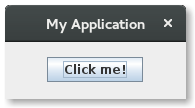
\includegraphics[width=3cm]{pictures/button-swing.png}
	\end{figure}
	\end{columns}

	\pause \vspace{0.5cm}
	\begin{figure}
	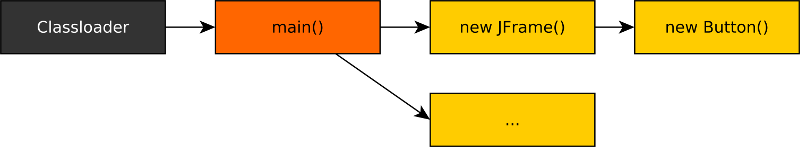
\includegraphics[width=\textwidth]{pictures/call-hierachy-swing.png}
	\end{figure}
\end{frame}


\begin{frame}[c]
	\frametitle{Android App}
	\begin{columns}[t]
	\column{.7\textwidth}
	\begin{itemize}
	\item nur ein Fenster kann angezeigt werden \pause
	\item weniger Prozessor- und Akkuleistung \pause \\
		$\Rightarrow$ System muss mit Resourcen haushalten \pause
	\item stärkere Systemintegration \\ (Notifications, Sensoren,...) \pause
	\end{itemize}
	\vspace{0.2cm}
	$\Rightarrow$ \textbf{Activities} \\
	\hspace{1cm}Container für graphische Anwendungen \pause

	\column{.3\textwidth}
	\vspace{-1cm}
	\begin{figure}
	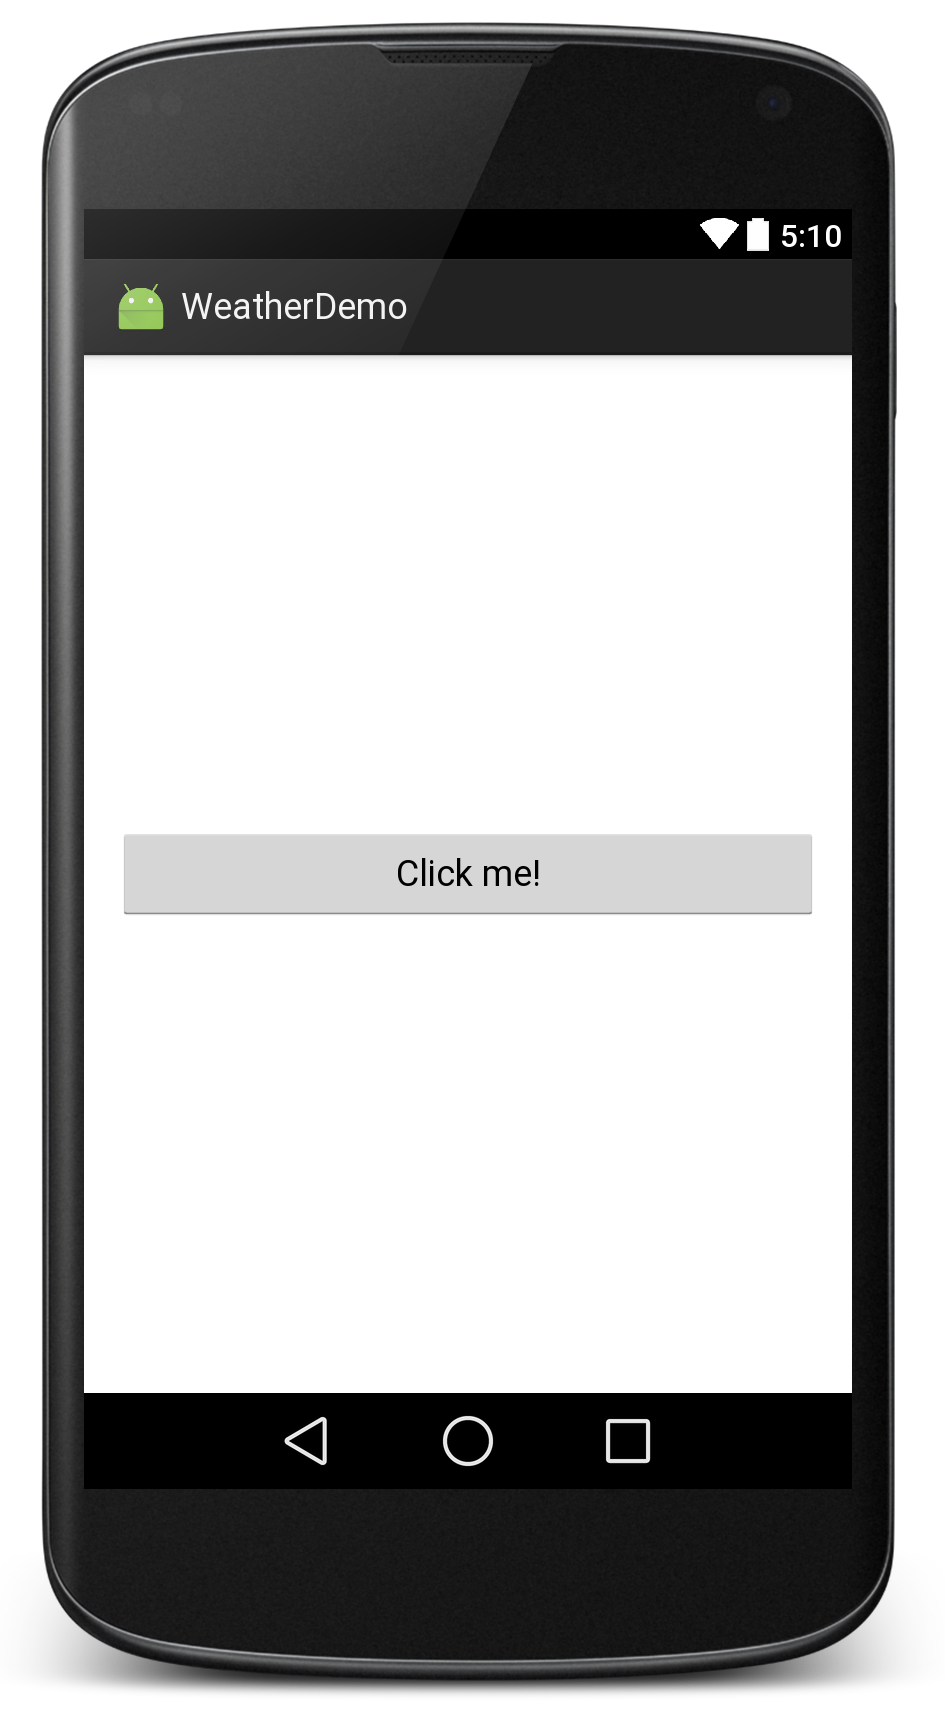
\includegraphics[height=6cm]{pictures/button-android-framed.png}
	\end{figure}
	\end{columns}
\end{frame}

\begin{frame}[c,fragile]
	\frametitle{Android Button App}
	\begin{lstlisting}
	class MainActivity extends Activity {
	    @Override
	    public void onCreate() {
	        //TODO add Button
	    }
	}
	\end{lstlisting}
	\pause \vspace{0.5cm}
	\begin{lstlisting}[language=XML]
	<manifest>
	  <application label="ButtonApp">
	    <activity name=".MainActivity" 
	              label="My Activity">
        ...
	</...>
	\end{lstlisting}
\end{frame}

\frame[c]{
	\frametitle{Inversion of control}
	\centering
	\textbf{Swing}
	\begin{figure}
	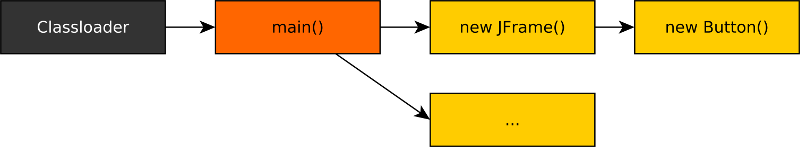
\includegraphics[width=0.8\textwidth]{pictures/call-hierachy-swing.png}
	\end{figure}
	\vspace{0.2cm}\pause
	\textbf{Android}
	\begin{figure}
	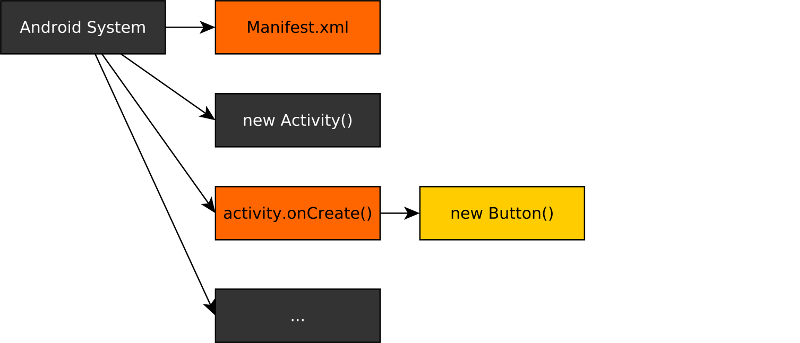
\includegraphics[width=0.8\textwidth]{pictures/call-hierachy-android.png}
	\end{figure}
}

\frame[c]{
	\frametitle{Activity Lifecycle}
	\begin{figure}
	\centering
	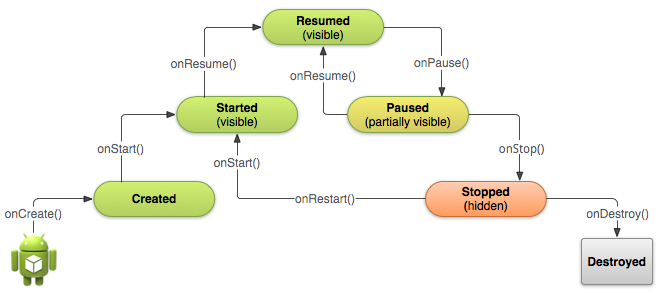
\includegraphics[width=\textwidth]{pictures/activity_lifecycle.png}
	\end{figure}
	\pause
	\begin{columns}
	\column{.5\textwidth}
	\textbf{onCreate()}
	\begin{itemize}
	\item initialize UI \pause
	\item start Animations \pause
	\item connect to Sensors \pause
	\end{itemize}
	\column{.5\textwidth}
	\textbf{onDestroy()}
	\begin{itemize}
	\item persist User Data \pause
	\item stop Animations \pause
	\item disconnect from Sensors
	\end{itemize}
	\end{columns}
}

\frame[t]{
	\frametitle{Intents...}
	\begin{itemize}[<+->]
		\item Hauptkommunikationsmittel zwischen Komponenten
		\item ... enthalten explizites oder implizites Ziel \\
			\textit{z.B. ``Öffne Facebook'' oder ``Sende Mail''}
		\item ... können noch weitere Daten enthalten \\
			\textit{z.B. Titel der Mail, URL einer Website, ...}
		\item ... werden vom System an das jeweilige Ziel weitergeleitet
	\end{itemize}
	\vspace{-0.5cm}
	\begin{columns}
	\column{.2\textwidth}
	\column{.3\textwidth}
	\begin{figure}
	\includegraphics[height=3cm]<5->{pictures/implicit-intent-hierarchy.pdf}
	\end{figure}
	\pause
	\column{.3\textwidth}
	\begin{figure}
	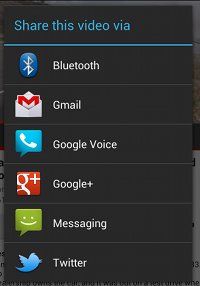
\includegraphics[height=3cm]{pictures/intent-choser.png}
	\end{figure}
	\column{.2\textwidth}
	\end{columns}
}
\section{GUI}
% Möglichst schlechtes Beispiel finden...
\frame{
	\frametitle{GUI}
	\vspace{-2mm}
	\begin{center}
		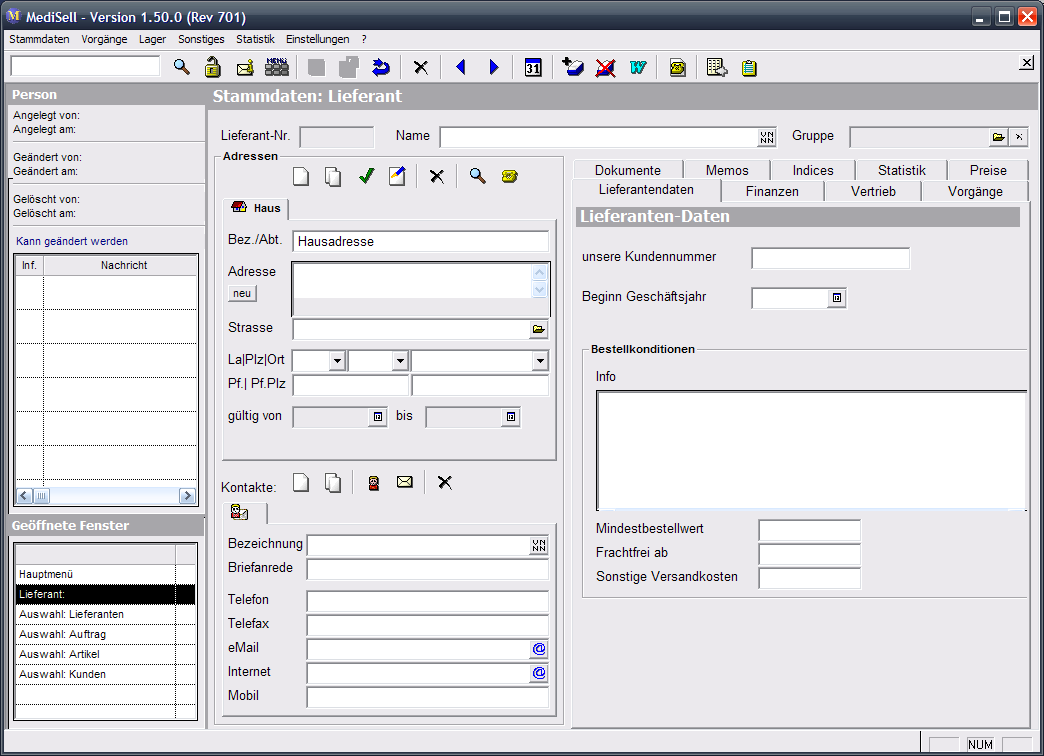
\includegraphics[width=.9\textwidth]{pictures/bad_gui_2.png}
	\end{center}
}
\frame{
	\frametitle{GUI}
	\vspace{-2mm}
	\begin{center}
		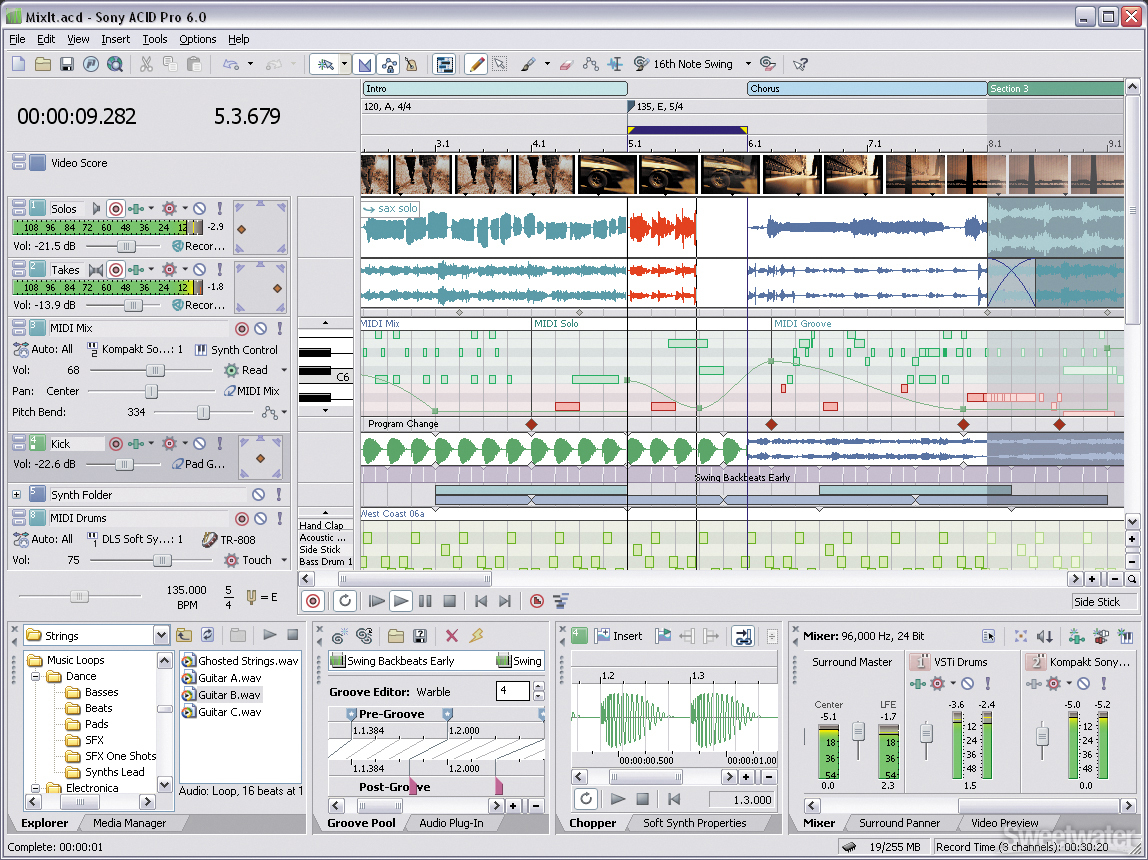
\includegraphics[width=.9\textwidth]{pictures/bad_gui_1.jpg}
	\end{center}
}
\frame{
	\frametitle{GUI}
	\vspace{-2mm}
	\begin{center}
		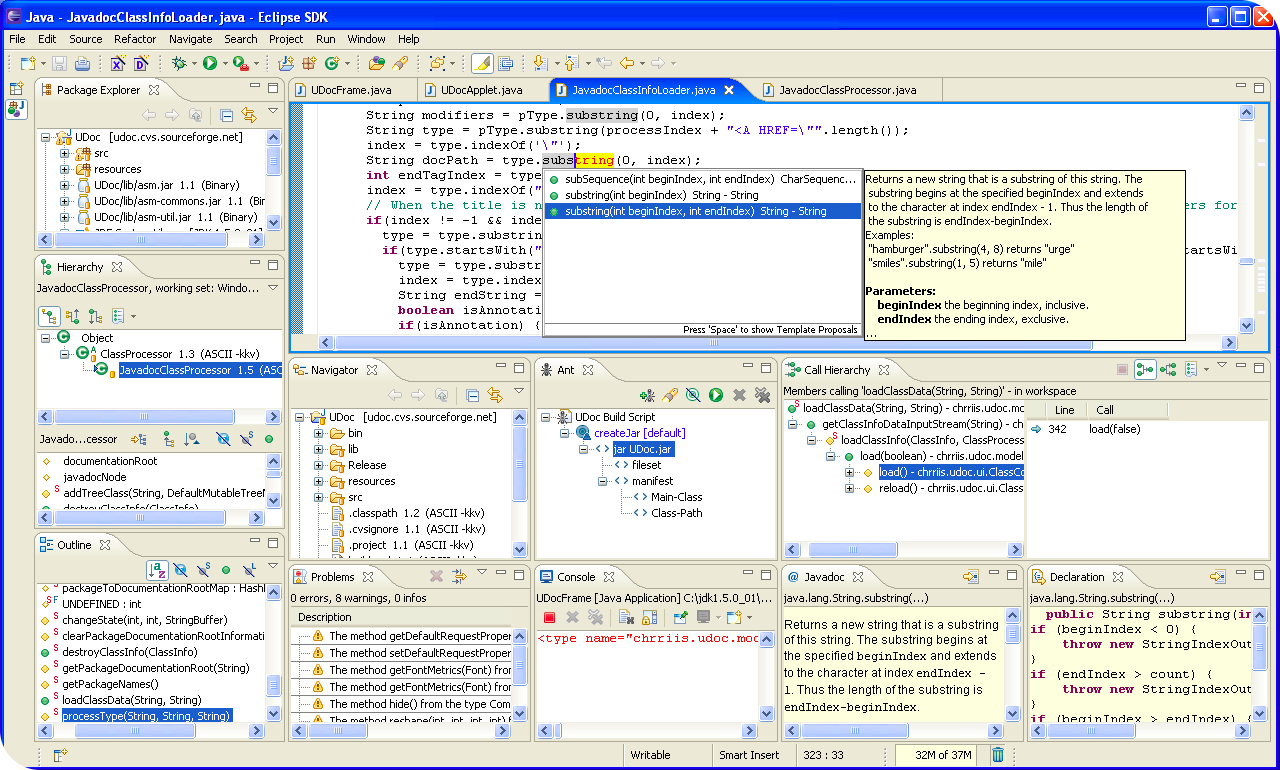
\includegraphics[width=.9\textwidth]{pictures/bad_gui_3.png}
	\end{center}
}
\frame{
	\frametitle{GUI}
	\vspace{-2mm}
	\begin{center}
		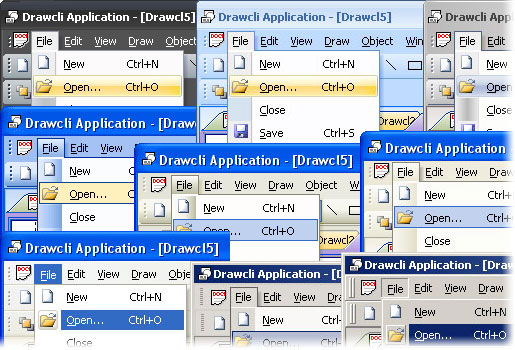
\includegraphics[width=.9\textwidth]{pictures/klickibunti.jpeg}
	\end{center}
}
\frame{
	\frametitle{Besonderheiten bei Smartphones/Tablets}
	\vspace{5mm}
	\begin{itemize}
		\item kleiner Bildschirm \pause
		\vspace{2mm}
		\item Touch-Bedienung \pause
		\vspace{2mm}
		\item verschiedene Größen, Auflösungen und Formate \newline \pause 
		\quad \( \implies \) Größenangaben in px oder cm ungeeignet \pause
		\vspace{2mm}
		\item Drehen des Bildschirms \pause
		\vspace{2mm}
		\item Anwendungskontext (draußen, im Gehen, etc.)
		\vspace{2mm}
		\item \dots
	\end{itemize}
	\vspace{2mm}
	\large{\( \implies \) abstrakte Beschreibung der GUI in XML}
	% ähnlich wie JavaFX, C#, etc.
}

\begin{frame}[fragile]
	\frametitle{XML}
	\vspace{-2mm}
	\begin{lstlisting}[language=XML]
		<Button
		    android:id="@+id/buttonRefresh"
		    android:layout_width="match_parent"
		    android:layout_height="60dp"
		    android:textSize="20sp"
		    android:text="Refresh" />
     \end{lstlisting}
     \pause
     \vspace{-9mm}
     \begin{center}
     	
\includegraphics[width=6cm]{pictures/buttonRefresh.png}
     \end{center}
     \pause
     \vspace{-5mm}
     \begin{itemize}
     	\item \verb|60dp| \textrightarrow \ density-independent pixels \newline
     	\quad \( \implies \) 1 Pixel auf 160 dpi Screen \pause
     	\vspace{2mm}
     	\item \verb|20sp| \textrightarrow \ scale-independent pixels \newline
     	\quad \( \implies \) persönliche Skalierung des Users
     \end{itemize}
\end{frame}

\begin{frame}[fragile]
	\frametitle{XML}
	\vspace{-2mm}
	\begin{lstlisting}[language=XML]
		<TextView
		    android:id="@+id/textViewTemperature"
		    android:layout_width="wrap_content"
		    android:layout_height="wrap_content"
		    android:textSize="50sp"
		    android:text="23 C" />
     \end{lstlisting}
     \pause
     \vspace{-9mm}
     \begin{center}
     	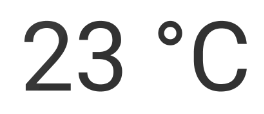
\includegraphics[width=2cm]{pictures/textViewTemperature.png}
     \end{center}
     \pause
     \vspace{-5mm}
     \begin{itemize}
     	\item \verb|wrap_content| \textrightarrow \ Breite/Höhe passt auf Inhalt \pause
     	\vspace{2mm}
     	\item \verb|match_parent| \textrightarrow \ Breite/Höhe passt auf Rahmen
     \end{itemize}
\end{frame}

\begin{frame}[fragile]
	\frametitle{Layouts}
	\vspace{-2mm}
	\begin{lstlisting}[language=XML]
		<LinearLayout
		    android:layout_width="match_parent"
		    android:layout_height="match_parent"
		    android:orientation="vertical" >

		    <TextView
		        ... />
		    <TextView
		        ... />

		</LinearLayout>
    \end{lstlisting}
\end{frame}

\begin{frame}[fragile]
	\frametitle{Layouts}
	\vspace{-2mm}
	\begin{lstlisting}[language=XML]
		<RelativeLayout
		    android:layout_width="match_parent"
		    android:layout_height="match_parent" >

		    <TextView
		        android:id="@+id/textView1"
		        android:layout_alignParentTop="true"
		        android:layout_centerHorizontal="true"
		        ... />
		    <TextView
		        android:id="@+id/textView2"
		        android:layout_below="@id/textView1"
		        android:layout_centerHorizontal="true"
		        ... />
		</RelativeLayout>
    \end{lstlisting}
\end{frame}

\begin{frame}[fragile]
	\frametitle{Layouts}
	\vspace{-2mm}
	\begin{lstlisting}[language=XML]
		<TableLayout
		    android:layout_width="match_parent"
		    android:layout_height="match_parent" >

		    <TableRow>
		        <TextView
		        ... />
		        <TextView
		        ... />
		    </TableRow>

		    <TableRow> ... </TableRow>

		</TableLayout>
    \end{lstlisting}
\end{frame}

\begin{frame}[fragile]
	\frametitle{Zugriff in Java}
	\begin{lstlisting}[language=Java]
		protected void onCreate(Bundle bundle) {
		    super.onCreate(bundle);

		    // define the layout for this activity
		    setContentView(R.layout.activity_main);
		    
		    // get a reference to the view elements
		    buttonRefresh = (Button)
		        findViewById(R.id.buttonRefresh);
		    textViewTemperature = (TextView)
		        findViewById(R.id.textViewTemperature);
		}
    \end{lstlisting}
\end{frame}

\begin{frame}[fragile]
	\frametitle{Zugriff in Java}
	\begin{lstlisting}[language=Java]
		// manipulate the UI
		textViewTemperature.setText("30")

		//react to UI actions
		buttonRefresh.setOnClickListener(
		    new View.OnClickListener() {
		        public void onClick(View v) {
		            //refresh
		        }
		    });
    \end{lstlisting}
\end{frame}



	% TODO

	% Übertriebenes Klickibunti-Bild
	% GUI wird in XML definiert
	% In Java holt man sich Referenzen darauf und kann es dann manipulieren
	% Layouts:
		% LinearLayout
		% TableLayout
		% RelativeLayout

\section{Sensoren}
\frame{
	\frametitle{Sensoren} \pause
	\vspace{5mm}
	\begin{itemize}
		\item Physikalisch:
		\begin{itemize} 
			\item GPS
			\vspace{2mm}
			\item Accelerometer/Beschleunigung
			\vspace{2mm}
			\item Helligkeit
			\vspace{2mm}
			\item Mikrofon	
		\end{itemize}
		\vspace{3mm}
		\item Virtuell:
		\begin{itemize} 
			\item Schrittzähler
			\vspace{2mm}
			\item Lineare Beschleunigung
			\vspace{2mm}
			\item Lage/Rotation
		\end{itemize}
	\end{itemize}
}

\begin{frame}[fragile]
	\frametitle{GPS}
	\vspace{-3mm}
	\begin{lstlisting}[language=Java]
		LocationListener listener = new LocationListener() {
		    public void onLocationChanged(Location loc){
		    	// fetch the weather using the provided
		    	// location
		        fetchWeather(loc.getLatitude(),
		            loc.getLongitude()); 
		    }

		    public void onStatusChanged(...) {...}
		    public void onProviderEnabled(...) {...}
		    public void onProviderDisabled(...) {...}
		};
    \end{lstlisting}	
	
\end{frame}

\begin{frame}[fragile]
	\frametitle{GPS}
	\begin{lstlisting}[language=Java]
		// get a location manager
		LocationManager locationManager =
		    (LocationManager) getSystemService(
		        LOCATION_SERVICE);

		// request a single location update
		locationManager.requestSingleUpdate(
		    LocationManager.GPS_PROVIDER, listener,
		        getMainLooper());
		// getMainLooper() used for executing the
		// callback (ignore for now)
    \end{lstlisting}
\end{frame}

\begin{frame}[fragile]
	\frametitle{GPS}
	\begin{lstlisting}[language=Java]
		// request continuous location updates each
		// hour with a minimum distance of 1 km 
		locationManager.requestLocationUpdates(
		    LocationManager.GPS_PROVIDER,
		        360000000, 1000, listener);
    \end{lstlisting}
    \pause
	\begin{lstlisting}[language=Java]
		// just get the last known location
		Location location = locationManager.
		    getLastKnownLocation(
		        LocationManager.PASSIVE_PROVIDER);
    \end{lstlisting}    
\end{frame}








\section{Threading}
\frame[t]{
	\frametitle{Threading Problems}
	\begin{figure}
	\includegraphics[width=\textwidth]<1>{pictures/errors-1.png}
	\includegraphics[width=\textwidth]<2>{pictures/errors-2.png}
	\includegraphics[width=\textwidth]<3>{pictures/errors-3.png}
	\end{figure}
}

\frame[c]{
	\frametitle{Android Threading}
	\begin{itemize}
	\item \textbf{Android UIs sind single-threaded!} \pause \medskip
	\item Tasks auf dem UI Thread blockieren die App \\
		$\Rightarrow$ \emph{App-Not-Responding} Dialog wird angezeigt \pause \medskip
	\item IO ist im UI Thread verboten \\
		$\Rightarrow$ sonst \texttt{NetworkOnMainThreadException} \pause \medskip
	\item UI kann nur vom UI Thread aus aktualisiert werden  \\
		$\Rightarrow$ sonst \texttt{CalledFromWrongThreadException} \pause \medskip
	\item Threads, die von einer Activity aus gestartet wurden, \\ werden beendet sobald die Acitvity geschlossen wird \pause \medskip
	\item Activities (und damit auch alle Threads) werden neu gestartet, \\ wenn der Bildschirm gedreht wird
	\end{itemize}
}

\frame[c]{
	\frametitle{Alternativen}
	\begin{itemize}
	\item Starte anderen Thread und aktualisiere UI mit \texttt{Activity.runOnUiThread(Runnable)} \\ \pause \smallskip
		$\Rightarrow$ \emph{Kommunikation mit UI trotzdem sehr aufwändig}\pause \bigskip
	\item Verwende \texttt{AsyncTask}  \pause
		\begin{itemize}
		\item \texttt{onPre/PostExecute()} auf dem UI Thread \pause
		\item \texttt{doInBackground(...)} asynchron \pause
		\item Parameter und Rückgabewerte \pause
		\item Fortschritt mit \texttt{onProgressUpdate(...)} \pause
		\item Abbrechen mit \texttt{cancel()} \pause \smallskip
		\end{itemize}
		$\Rightarrow$ \emph{wird immernoch zusammen mit Activity beendet}
	\end{itemize}
}

\begin{frame}[c]
	\frametitle{Services}
	\begin{itemize}
	\item Eigenständige Komponente neben Activities \pause \medskip
	\item läuft über längere Zeit im Hintergrund \pause \medskip
	\item asynchron und unabhängig von Activities \pause \medskip
	\item Aufgabenbereiche
		\begin{itemize}
		\item Dateiup- und download \pause
		\item Datensynchronisierung \pause
		\item Notifications \pause
		\item Datenlogging \pause
		\item Zeitgesteuerte Abläufe
		\item ...
		\end{itemize}
	\end{itemize}
\end{frame}

\begin{frame}[c]
	\frametitle{Arten von Services}
	\begin{itemize}
	\item \textbf{IntentService}
		\begin{itemize}
		\item Arbeitspakete in Form von Intents \pause
		\item arbeitet der Reihe nach ab und beendet sich automatisch \pause
		\item Wertrückgabe in Form von Intents \pause
		\end{itemize}

	\bigskip
	\item \textbf{Started Service}
		\begin{itemize}
		\item durch Intent(s) gestartet \pause
		\item unbeschränkte Lebensdauer \pause
		\end{itemize}

	\bigskip
	\item \textbf{Bound Service}
		\begin{itemize}
		\item hält Verbindung mit Activities, mit diesen direkte Kommunikation \pause
		\item Lebenszeit an die der Activities gebunden
		\end{itemize}
	\end{itemize}
\end{frame}




% \frame{
%   \frametitle{Ablauf}
%   \tableofcontents
% }

% \include{begruessung}
% \include{fachschaft}
% \include{Quitschie}
% \include{tipps}
% \include{lageplan}
% \include{tueten}


\end{document}